\section{Filter}\script{31}
Ideale Filter sind akausal und daher nicht realisierbar.

\subsection{Hochpassfilter}
Ein High-pass Filter (HPF) dämpft unterhalb von $f_c$ alle Frequenzanteile vollständig. Die Bandbreite $B$ eines Hochpassfilters ist undefiniert, da der Durchlassbereich auf der Frequenzachse gegen hogh Frequenzen hin offen und somit unendliche gross ist.
\begin{center}
	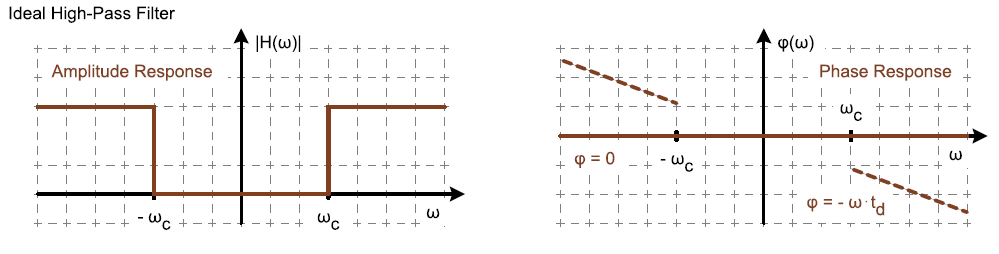
\includegraphics[width=0.8\columnwidth]{Images/hochpass}
\end{center}


\subsection{Tiefpassfilter}
Ein Low-pass Filter (LPF) dämpft oberhalb von $f_c$ alle Frequenzanteile vollständig. Die Bandbreite $B$ eines Tiefpassfilters erstreckt sich von Frequenz $0Hz$ bis Eckfrequenz $f_c$, d.h. $B = f_c$
\begin{align*}
	\left|H(2\pi f_{c})\right| &= \frac{\sqrt{2}}{2}\cdot \left|H(0)\right| \\
	\left|H(2\pi f_{c})\right|_{dB} &= \left|H(0)\right|_{dB} - 3dB
\end{align*}

\begin{center}
	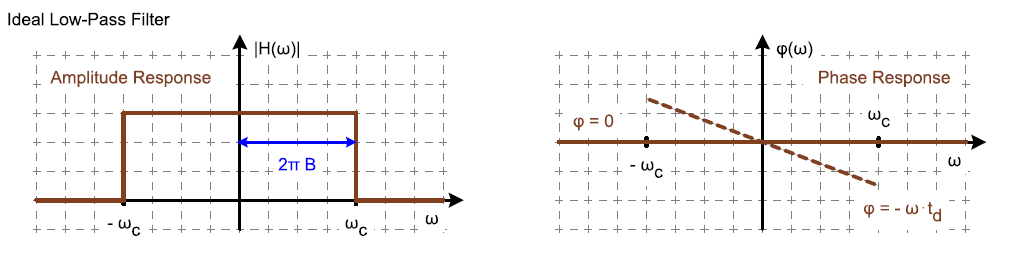
\includegraphics[width=0.8\columnwidth]{Images/tiefpass}
\end{center}

\subsection{Bandpassfilter}
Die Bandbreite $B$ eines BPF erstreckt sich von unterer Eckfrequenz $f_{cl}$ bis zur oberen Eckfrequenz $f_{cu}$, d.h. $B = f_{cu} - f_{cl}$. Bzw:
\begin{align*}
	\left|H(2\pi f_{cl})\right| &= \left|H(2\pi f_{cu})\right| = \frac{\sqrt{2}}{2}\cdot \left|H(2\pi f_{center})\right| \\
	\left|H(2\pi f_{cl})\right|_{dB} &= \left|H(2\pi f_{cu})\right|_{dB} = \left|H(2\pi f_{center})\right|_{dB} - 3dB
\end{align*}
\begin{center}
	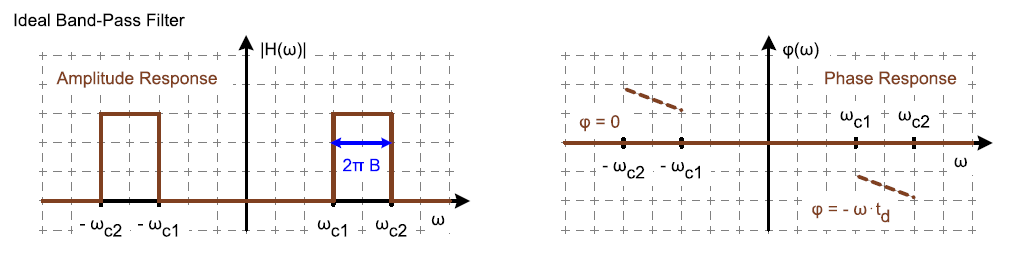
\includegraphics[width=0.8\columnwidth]{Images/bandpass}
\end{center}

\noindent Schmalbandiges Filter $B \ll f_{center}$ und Breitbandiges Filter $B \approx f_{center}$.

\subsection{Hilbert-Transformation}\label{hilbert}
Die Hilbert-Transformation oder auch \textbf{Quadraturfilter} verschiebt Imaginärteil gegenüber Realteil um 90° bzw $\pi/2$ 
\begin{align*}
	\hat{x}(t) &= \frac{1}{\pi}\int_{-\infty}^{\infty}\frac{x(\tau)}{t - \tau}d\tau \\
	\hat{X}(\omega) &= -j \cdot \sgn(\omega) \cdot X(\omega)
\end{align*}

\begin{center}
	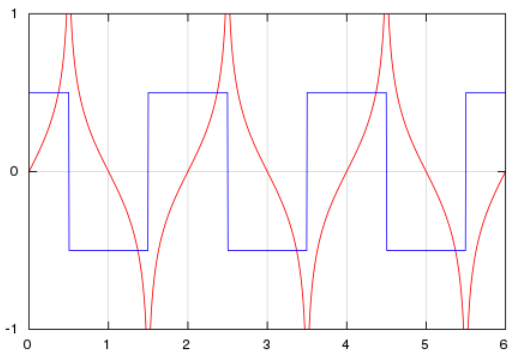
\includegraphics[width=0.6\columnwidth]{Images/hilbert}
\end{center}